\documentclass{article}
\usepackage[margin=1in]{geometry}

\usepackage{tikz}


\newcommand{\diagram}{
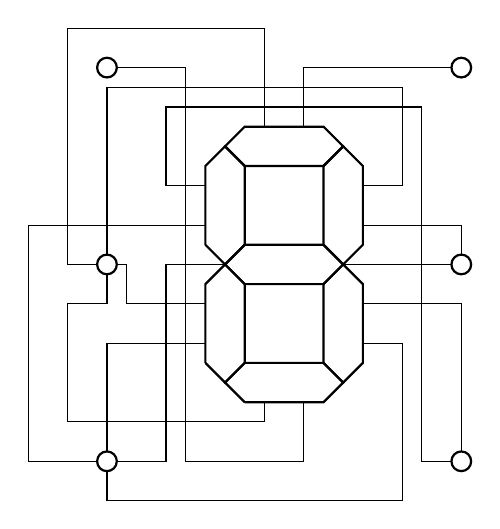
\begin{tikzpicture}[scale=0.25]
%\draw[color=black!20,step=1] (-6,-4) grid (14,18);
\begin{scope}
\draw[thick] (2,0) -- (6,0) -- (7,1) -- (6,2) -- (2,2) -- (1,1) -- (2,0);
\end{scope}
\begin{scope}[shift={(0,6)}]
\draw[thick] (2,0) -- (6,0) -- (7,1) -- (6,2) -- (2,2) -- (1,1) -- (2,0);
\end{scope}
\begin{scope}[shift={(0,12)}]
\draw[thick] (2,0) -- (6,0) -- (7,1) -- (6,2) -- (2,2) -- (1,1) -- (2,0);
\end{scope}
\begin{scope}
\draw[thick] (0,2) -- (1,1) -- (2,2) -- (2,6) -- (1,7) -- (0,6) -- (0,2);
\end{scope}
\begin{scope}[shift={(6,0)}]
\draw[thick] (0,2) -- (1,1) -- (2,2) -- (2,6) -- (1,7) -- (0,6) -- (0,2);
\end{scope}
\begin{scope}[shift={(0,6)}]
\draw[thick] (0,2) -- (1,1) -- (2,2) -- (2,6) -- (1,7) -- (0,6) -- (0,2);
\end{scope}
\begin{scope}[shift={(6,6)}]
\draw[thick] (0,2) -- (1,1) -- (2,2) -- (2,6) -- (1,7) -- (0,6) -- (0,2);
\end{scope}
\draw (-5,-3) -- (-2,-3) -- (-2,7) -- (1,7);
\draw (-5,-3) -- (-9,-3) -- (-9,9) -- (0,9);
\draw (-5,-3) -- (-5,-5) -- (10,-5) -- (10,3) -- (8,3);
\draw (-5,-3) -- (-5,3) -- (0,3);
\draw (-5,7) -- (-5,5) -- (-7,5) -- (-7,-1) -- (3,-1) -- (3,0);
\draw (-5,7) -- (-7,7) -- (-7,19) -- (3,19) -- (3,14);
\draw (-5,7) -- (-4,7) -- (-4,5) -- (0,5);
\draw (-5,7) -- (-5,16) -- (10,16) -- (10,11) -- (8,11);
\draw (-5,17) -- (-1,17) -- (-1,-3) -- (5,-3) -- (5,0);
\draw (13,17) -- (5,17) -- (5,14);
\draw (13,7) -- (7,7);
\draw (13,7) -- (13,9) -- (8,9);
\draw (13,-3) -- (11,-3) -- (11,15) -- (-2,15) -- (-2,11) -- (0,11);
\draw (13,-3) -- (13,5) -- (8,5);
\draw[thick,fill=white] (-5,-3) circle (0.5);
\draw[thick,fill=white] (-5,7) circle (0.5);
\draw[thick,fill=white] (-5,17) circle (0.5);
\draw[thick,fill=white] (13,-3) circle (0.5);
\draw[thick,fill=white] (13,7) circle (0.5);
\draw[thick,fill=white] (13,17) circle (0.5);
\end{tikzpicture}
}

\begin{document}

\begin{center}
\diagram \hspace{3em} \diagram

\vspace{3em}

\diagram \hspace{3em} \diagram
\end{center}

\newpage

Flavortext:

The Designer's favorite number is said to be
the digit 8. As they would say, "It's only logical."

- AND: Both active.

- NAND: Something inactive.

- OR: Something active.

- NOR: Both inactive.

- XOR: Both different.

- IFF: Both same.

One of the passwords seems to be related to this number,
but it can only be revealed once you consider the meaning
of an "unseen" GRAY.

\begin{center}
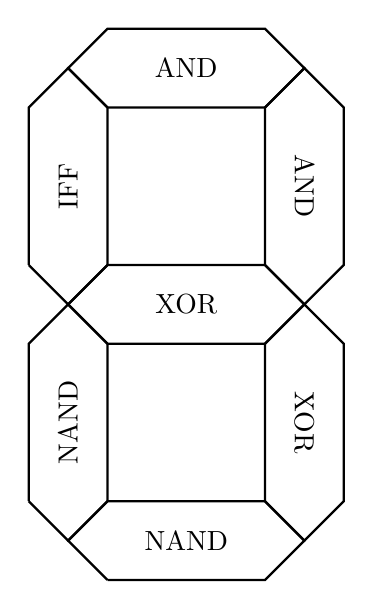
\begin{tikzpicture}[scale=0.5]
\begin{scope}
\draw[thick] (2,0) -- (6,0) -- (7,1) -- (6,2) -- (2,2) -- (1,1) -- (2,0);
\node at (4,1) {NAND};
\end{scope}
\begin{scope}[shift={(0,6)}]
\draw[thick] (2,0) -- (6,0) -- (7,1) -- (6,2) -- (2,2) -- (1,1) -- (2,0);
\node at (4,1) {XOR};
\end{scope}
\begin{scope}[shift={(0,12)}]
\draw[thick] (2,0) -- (6,0) -- (7,1) -- (6,2) -- (2,2) -- (1,1) -- (2,0);
\node at (4,1) {AND};
\end{scope}
\begin{scope}
\draw[thick] (0,2) -- (1,1) -- (2,2) -- (2,6) -- (1,7) -- (0,6) -- (0,2);
\node[rotate=90] at (1,4) {NAND};
\end{scope}
\begin{scope}[shift={(0,6)}]
\draw[thick] (0,2) -- (1,1) -- (2,2) -- (2,6) -- (1,7) -- (0,6) -- (0,2);
\node[rotate=90] at (1,4) {IFF};
\end{scope}
\begin{scope}[shift={(6,0)}]
\draw[thick] (0,2) -- (1,1) -- (2,2) -- (2,6) -- (1,7) -- (0,6) -- (0,2);
\node[rotate=-90] at (1,4) {XOR};
\end{scope}
\begin{scope}[shift={(6,6)}]
\draw[thick] (0,2) -- (1,1) -- (2,2) -- (2,6) -- (1,7) -- (0,6) -- (0,2);
\node[rotate=-90] at (1,4) {AND};
\end{scope}
\end{tikzpicture}
\end{center}

\end{document}
